\part{Smart Grid}
\chapter[Smart Grid]{Smart Grid}

\section{Introdução}

\subsection{Resumo}
Smart Grid (Rede inteligente) é um sistema de controle inteligente da energia elétrica, que é utilizado em um determinado local, com o objetivo principal de otimizar o consumo de energia elétrica e promover o controle por meio de ações inteligentes. Essa otimização da rede pode se dar pela utilização da rede já presente, promovendo apenas automações e controles, ou pela utilização de uma geração distribuída de energia com a adição de fontes renováveis aliadas à automação e controle. Busca-se, com o uso dessas tecnologias, proporcionar um uso eficiente, sustentável e racional dos recursos energéticos, podendo trazer benefícios financeiros ou não.

Esses sistemas permitem a implementação de duas formas principais de geração distribuída: \textit{On grid} e \textit{Off Grid}. Os sistemas On grid são ligados à rede elétrica e a energia gerada é armazenada na rede de distribuição. A economia de eletricidade se dá por meio de descontos na fatura de energia elétrica ou pela compensação. Caso a eletricidade gerada não for o suficiente, a rede elétrica externa compensa o consumo excedente. O sistema Off Grid, ou sistema isolado, não é conectado à rede elétrica externa, sendo utilizável para uso local e isolado de rede elétrica, abastecendo diretamente os aparelhos que utilizarão a energia. Além disso, sistemas Off Grid necessitam de unidades de armazenamento local, tais como baterias, visto que a variação na fonte geradora não pode causar alterações na corrente elétrica local. 

As tecnologias que compõem um sistema Smart Grid possuem complexidade elevada e um alto nível de integração entre seus diversos componentes, que podem ser divididos em quatro importantes setores que se interagem. São eles: o sensoriamento e controle, transmissão de dados, automatização e TI e a análise avançada dos dados. Eles estão intimamente ligados em todas as aplicações no sistema e procuram encontrar formas mais efetivas para evoluir continuamente o sistema, não ficando presos às primeiras modificações. O sistema inteligente é monitorado em todas as suas fases, permitindo um maior controle sobre o sistema e podendo ser identificado à pronta mão, onde estão os maiores problemas e riscos ao sistema, dando uma maior segurança aos usuários.


\subsection{Sensoriamento e controle}
Sensores e transdutores podem ser caracterizados como todo e qualquer dispositivo capaz de analisar grandezas físicas e convertê-las em um indicativo visível ou em grandezas mensuráveis de tensão e corrente, no caso de transdutores. Portanto, os sensores e transdutores são dispositivos muito utilizados em circuitos eletroeletrônicos para o monitoramento, transmissão de dados, automação e controle de ações a partir de condições físicas externas ou internas a esses sistemas, tais como tensão, corrente elétrica, potência, temperatura, pressão, radiações eletromagnéticas, temperatura, dentre outros \cite{svoboda2008introduccao}.

Diversos sensores são utilizados para o monitoramento e controle. Os sensores de linha, que analisam características elétricas da rede elétrica (tensão, corrente, defasagem, potência), são utilizados na construção de medidores inteligentes. \textbf{Sensores de temperatura} e piranômetros, que medem a irradiação solar e sensações térmicas, são sensores geralmente utilizados para realizar análises gráficas quanto às condições ambientais externas e internas do sistema, os quais podem ser guardados em bancos de dados.

Dentre os sensores a serem utilizados na automação interna de sistemas Smart Grids destacam-se os sensores de luminosidade, sensores infravermelho e sensores de presença, que serão descritos posteriormente.

Além desses tipos de sensores, vale ressaltar os \textbf{sensores de comunicação} e transmissão de dados, que constituem-se de sensores fotoelétricos, infravermelhos ou por meio de sensores ultrassonoros.


\subsection{Análise avançada de dados}
\begin{quotation}
Aplicações avançadas que permitem aos operadores, projetistas de redes e executivos analisarem e extraírem informações úteis da rede de forma funcional e flexível. Aqui se incluem as técnicas de visualização de grande quantidade de dados, os quais são reduzidos a formatos visuais de fácil entendimento, softwares capazes de oferecer múltiplas opções para o operador da rede tomar uma ação quando requerida e simuladores para treinamento operacional e análises de casos.
\end{quotation}

Consiste, portanto, em uma solução de software avançada que controla e armazena dados referentes aos sensores de controle, tais como os de temperatura e de linha. Para essa análise a recepção de dados é feita a partir de hardwares, por meio da comunicação sem fio ou serial por meio de processadores ou microcontroladores embarcados.


\subsection{Automação e TI}
Dentro de uma estrutura Smart Grid, os componentes de automação e TI (tecnologias da informação) permitem diagnósticos rápidos e soluções precisas para interrupções na rede ou grandes desligamentos. Essas tecnologias baseiam-se e contribuem para as demais partes, tais como sensores, comunicação, análise de dados e fontes de energia. Sistemas nessa área incluem agentes inteligentes distribuídos, algoritmos e supercomputadores, sistemas SCADA – Supervisory Control and Data Acquisition, automação de subestações e resposta da demanda \cite{josesmartgrid}.

Sistemas SCADA constituem-se de soluções de software voltadas para a análise e exibiçao de dados por meio de uma interface de comunicação com o usuário em tempo real, o que permite a configuração e ajuste para resolução de problemas de forma visual e o monitoramento de processos. Tal solução baseia-se na tecnologia da informação, muitas vezes associado também à \textit{internet das coisas} (IoT). Possui uma vida útil finita, visto que a tecnologia de informação evolui de forma rápida, tornando o software defasado em alguns anos, tornando um desafio a aplicação dessa tecnologia em projetos de longa vida útil \cite{galloway2013introduction}.

A aplicação de agentes inteligentes em ambientes Smart Grid é comum, principalmente na medição do consumo de energia. Nessa vertente, existem dois conceitos ligados ao desenvolvimento de medidores inteligentes: AMR (Automated Meter Reading) e AMI (Advanced Metering Infrastructure).

AMR é um sistema de medidores inteligentes que transfere os dados armazenados pelos medidores eletrônicos de forma automatizada quando integrado a um sistema de processamento de dados. Ou seja, não se faz necessária a presença humana para a leitura da medição. AMI é uma evolução do AMR, pois além de prover os dados obtidos na medição, esse sistema também faz a análise da demanda. Esse processo requer um processamento de dados mais sofisticado, visto que a atuação é direta nas instalações do consumidor, permitindo o planejamento mensal de consumo \cite{kup2015estudo}.


\subsection{Transmissão de dados}
Dentro de um sistema, é essencial que todos os componentes se comuniquem de forma adequada para que tudo funcione corretamente. Para definir a melhor forma de se transmitir os dados, podemos analisar a distância física que eles precisam percorrer e a quantidade de bits por segundo que se deseja transmitir. A comunicação entre os componentes envolve também alguns aspectos minuciosos como os protocolos, que consistem em um conjunto de regras no processo de interpretação e transmissão de dados de um componente.  Dependendo dos sensores escolhidos, por exemplo, pode não ser tão simples elaborar essa linha de transmissão de forma efetiva. Será visto mais a frente que uma alternativa é utilizar um sistema já existente no mercado com suporte para diferentes tipos de componentes.

\section{Desenvolvimento}
Descritas as ferramentas utilizadas em soluções Smart Grids, propõe-se a integração das fontes renováveis, a automação das redes e processos, comunicação, controle e sensoriamento a partir da comparação de sistemas, de modo com que haja interconexão entre as diferentes vertentes. Para tanto, a seguir serão comparadas características de operações, compatibilidade com o restante do projeto e adaptabilidade ao local de instalação (FGA).

\subsection{Sensores de temperatura}
A utilização dos sensores de temperatura será baseada no monitoramento de ambientes e para automação interna (acionamento de exaustores/ventiladores) e no monitoramento de sobreaquecimento de equipamentos e condutores. Dentre os sensores térmicos existentes, diferenciam-se no funcionamento os termistores, termopares, termorresistores, eletrônicos e pirômetros. Termistores são compostos por dispositivos que variam a resistência elétrica em função da temperatura, que pode ser inversamente proporcional a ela (NTC) ou diretamente proporcional (PTC). Termopares consistem de uma junção de dois materiais de condutividades elétricas distintas pela qual irá passar uma corrente que provocará uma queda de tensão proporcional à temperatura de sua superfície. PT RTD são sensores cuja variação na resistência se dá por meio da dilatação do material, que é proporcional ao aumento de temperatura. Termosensores de circuitos integrados constituem de sensores compostos por diversos componentes de modo que a sua saída não necessita de muitos hardwares para o condicionamento do sinal \cite{thomazini2005sensores}.

A tabela abaixo ilustra os diferentes tipos de sensores e suas características de funcionamento.

\begin{figure}[!h]
	\centering
	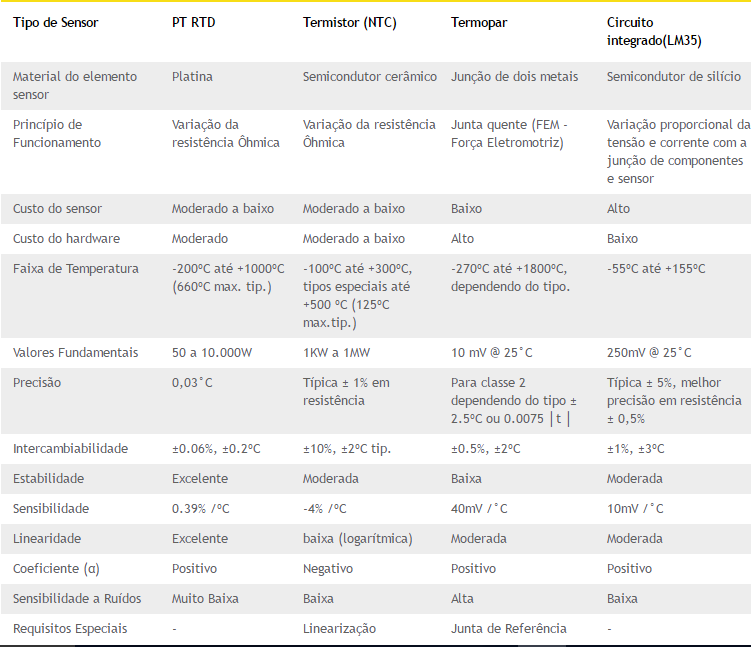
\includegraphics[width=1.0\textwidth]{figuras/tabelaSensoresTermicos.png}
	\caption{Tabela ilustrativa de sensores térmicos}
	\label{fig:sensorestermicos}
\end{figure}

Dentre os sensores listados na Figura \ref{fig:sensorestermicos}, conclui-se que os termistores serão utilizados para o gerenciamento de sobreaquecimentos, visto que a sua faixa de temperatura de trabalho não ultrapassa os limites do projeto e visto que a precisão de temperatura adquirida, que é um aspecto relevante no monitoramento de temperatura, é melhor em comparação com outros tipos de sensores.


\subsection{Sensores de presença}
Quanto ao projeto de Smart Grid, os sensores de presença serão fundamentais na diminuição do consumo de energia elétrica na Universidade no que diz respeito à automação interna dos prédios e salas. Propõe-se a automação de banheiros, pois as luzes ficam acesas em determinados momentos em que não há ninguém presente no local e em salas de aula, pelo mesmo motivo. Esses sensores têm como objetivo a automação interna de ambientes com alto fluxo de pessoas, onde funcionam tanto para o monitoramento ou quanto para o acionamento de lâmpadas/exaustores com a entrada ou saída de pessoas. Dentre os tipos de sensores de presença, destacam-se os modelos de parede, embutidos e os de teto. Na figura \ref{fig:sensorpresenca} é possível observar as diferenças e semelhanças entre os modelos.
\begin{figure}[!h]
	\centering
	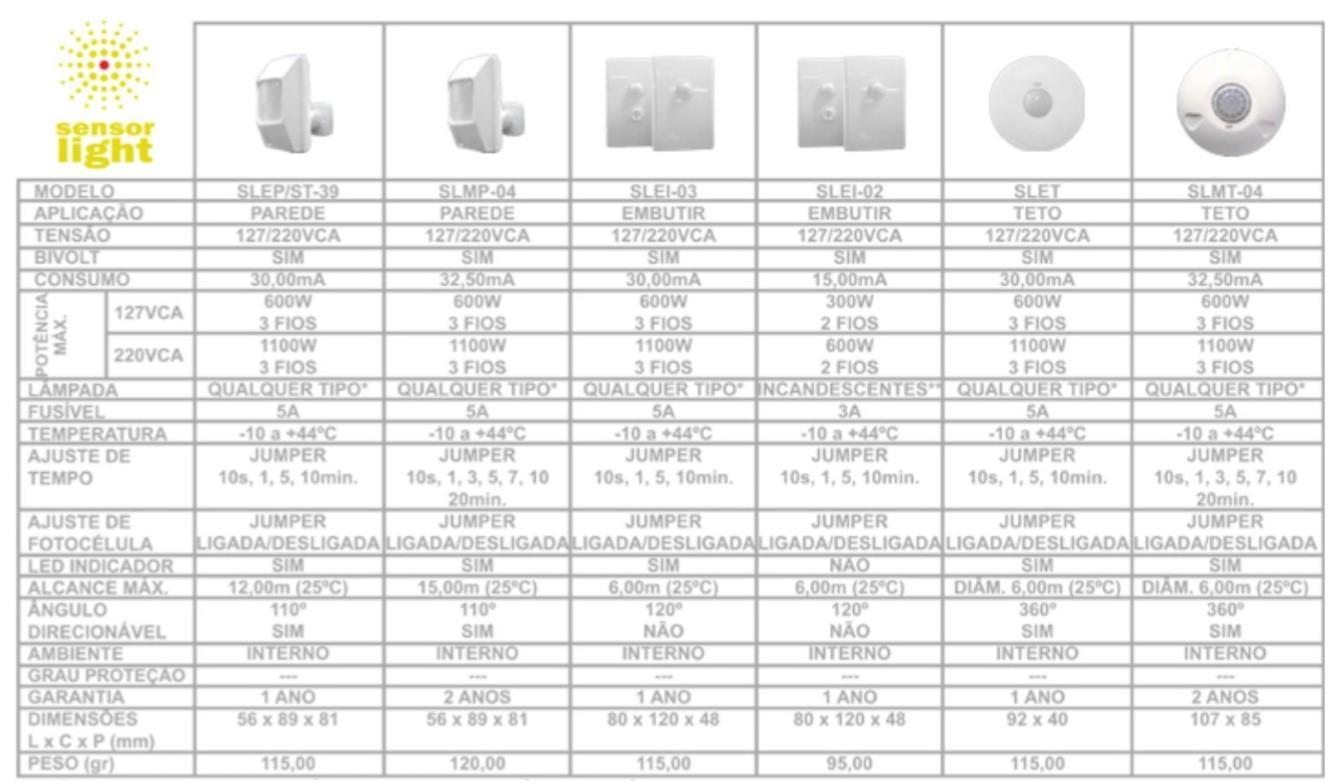
\includegraphics[width=1.0\textwidth]{figuras/tabelaSensorPresenca.png}
	\caption{Quadro comparativo dos modelos de sensores de presença}
	\label{fig:sensorpresenca}
\end{figure}

O sensor a ser utilizado no projeto será o modelo SLEP/ST-39, pois é o que utiliza um menor consumo de energia elétrica dentre os sensores de presenças comerciais listados acima. Como os ambientes em que vão ser utilizados os sensores são no geral salas com uma área relativamente pequena, o alcance deste sensor é o suficiente para esse projeto. 


\subsection{Sensores de comunicação}
Sensores de comunicação infravermelho são componentes que se baseiam na emissão e recepção de ondas eletromagnéticas. No Conceito de Smart Grid, sensores infravermelhos e ultrassonoros podem ser utilizados como meios de transmissão de dados a distâncias curtas, porém sensores ultrassonoros possuem distâncias limitadas e são destinados apenas para aplicações de detecção de passagem. A transmissão de dados por meio de sensores infravermelhos se dá de forma serial e depende do protocolo de comunicação desses sensores com os respectivos emissores. 

Dentre os sensores infravermelhos utilizados em comunicação e transmissão de dados, destacam-se os sensores PIN e os sensores AFD. Sensores PIN são sensores receptores fotossintéticos que tem a vantagem de se adaptar melhor às condições climáticas e ter uma vida útil maior, além de possuir um menor custo. Sensores AFD ou APD são sensores receptores fotossintéticos que fornecem uma melhor adaptação quanto ao ruído, mesmo que o seu custo de produção seja maior \cite{jose2002sistema}.

Diferenças entre os fotodiodos PIN e AFD:
\begin{figure}[!h]
	\centering
	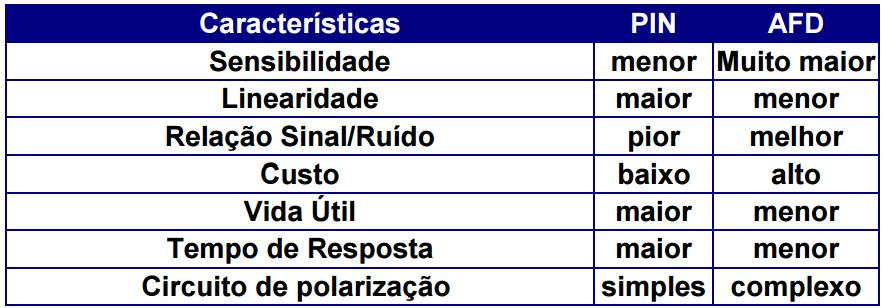
\includegraphics[width=0.7\textwidth]{figuras/tabelaSensorFotossintetico.png}
	\caption{Quadro comparativo entre sensores receptores fotossintéticos}
	\label{fig:sensorfotossintetico}
\end{figure}

Além das características técnicas referentes aos dois tipos de sensores presentes na Figura \ref{fig:sensorfotossintetico}, sensores APD possuem as desvantagens de  possuírem desempenho limitado por ruídos quânticos, a complexidade da estrutura, sensibilidade elevada quanto à variações de temperatura e uma menor fiabilidade.(ISCTE, Fotodetectores).

Além de fotodetectores tais como PIN e APD, em uma comunicação de dados infravermelhos, necessitam-se de emissores de radiação infravermelha. Dentre os principais tipos de emissores infravermelhos, caracterizam-se os LEDs infravermelhos (Light Emitting Diodes) e LDs (Lases Diodes) \cite{jose2002sistema}.

As principais diferenças são expostas no quadro presente na Figura \ref{fig:sensorinfravermelho}.
\begin{figure}[!h]
	\centering
	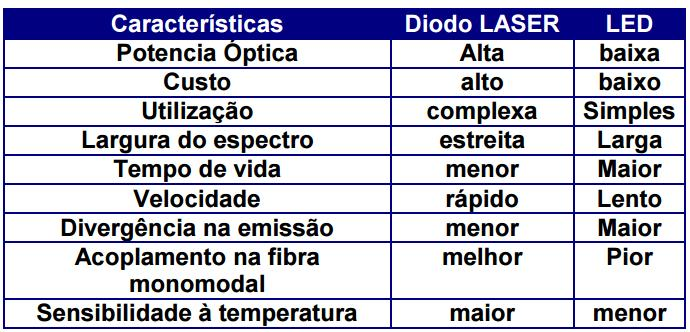
\includegraphics[width=0.7\textwidth]{figuras/tabelaSensorInfravermelho.png}
	\caption{Quadro comparativo entre sensores receptores fotossintéticos}
	\label{fig:sensorinfravermelho}
\end{figure}

Para fins de comunicação de distâncias médias de até 200m, e pela velocidade de resposta, a aplicação de diodos laser são mais eficientes e melhor adaptáveis para elementos de comunicação de dados devido também pela potência óptica associada a esses emissores.

A associação de elementos de emissão e recepção dos elementos tais quais descritos acima, referentes a radiações infravermelhas, é possível formar conjuntos de comunicação infravermelha. Para a comunicação entre prédios de dados referentes à análise de dados e controle, existem conjuntos de comunicação que atendem tanto os requisitos de emissão quanto os de recepção de dados. Conjuntos propostos pela Leuze Eletronic possuem comunicação serial, fotodetectores baseados em AFD e PIN e emissão por LDs. Dentre eles, destacam-se as séries  DDLS 500 E DDLS200.

DDLS 500 São dispositivos de transmissão de dados em tempo real e a distâncias médias. Permitem a tele-manutenção e a integração de redes PROFINET. Suas principais características são:
\begin{itemize}
\item Taxa de transmissão: 100Mbit/s;
\item Interfaces de comunicação: Ethernet, PROFINET, EtherCat;
\item Possibilidades de tele-manutenção por rede.
\end{itemize}

DDLS 200 São séries cujo foco é na eliminação de interferências, podendo operar a temperaturas altas e distâncias relativamente elevadas, cerca de 500m. Suas características principais são:
\begin{itemize}
\item Taxas de transferências : 2Mbit/s;
\item Interfaces de repeater integrada;
\item Elevada imunidade à luz ambiente;
\item Comunicação via PROFIBUS, interbus e CAN/DeviceNet.
\end{itemize}

Se levar em consideração que a distâncias entre prédios no estabelecimento a ser instalado não ultrapassariam 500m, além da não necessidade de velocidades rápidas de transmissão e, devido ao fato dos conjuntos DDLS 200 apresentarem características de resistências a temperatura e de luminosidade altas, que são fatores determinantes nos locais de instalações, foram escolhidos os modelos da série DDLS 200.

\subsection{Medidores Inteligentes}
Para a automatização do sistema Smart Grid a ser implementado na Faculdade Gama da Universidade de Brasília serão instalados medidores de energia inteligentes. Este novo conceito traz grandes vantagens que excedem as funcionalidades básicas dos medidores eletromecânicos ou eletrônicos convencionais e respondem às necessidades de melhoria de gestão e eficiência da medição, como detecção de fraude, corte e religamento remoto, comunicação bidirecional e medição à distância.

Em todos os prédios (UAC, UED E MESP) serão instalados medidores inteligentes por meio dos quais será possível monitorar a quantidade de energia elétrica que cada sistema produzir e, posteriormente, analisar os resultados obtidos por meio do compartilhamento dos dados. Segue o quadro comparativo entre dois possíveis modelos de medidores a serem utilizados:
\begin{figure}[!h]
	\centering
	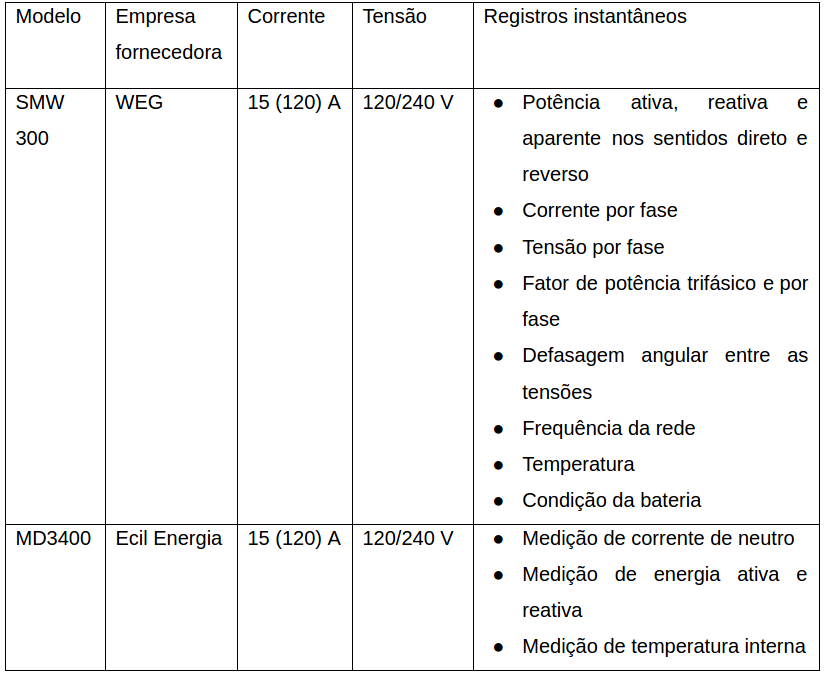
\includegraphics[width=1.0\textwidth]{figuras/quadroMedidoresInteligentes.png}
	\caption{Quadro de medidores inteligentes}
	\label{fig:medidoresinteligentes}
\end{figure}

O medidor SMW 300 possui uma gama maior de funcionalidades, e por isso será o modelo escolhido para o projeto. Tal equipamento é trifásico, ideal para a rede da FGA, e possui as seguintes características (Manual do Usuário - SMW): 
\begin{itemize}
\item Flexibilidade para mudança de tarifa convencional para tarifa branca com diferenciação tarifária;
\item Flexibilidade para mudança da comunicação (meio físico e protocolo);
\item Relé de corte e religa integrado;
\item Relógio de tempo real alimentado por bateria e supercapacitor, com monitoramento individual; 
\item Memória de massa integrada para registro de até 37 dias de informações;
\item Flexibilidade de configuração dos dados a serem enviados via comunicação e apresentados no display;
\item Mecanismos de segurança para garantia de sigilo e integridade, baseado na autenticação e criptografia de dados;
\item Atualização local ou remota do firmware da metrologia ou comunicação, com implementação de segurança contra acesso mal intencionado.
\end{itemize}
\begin{figure}[!h]
	\centering
	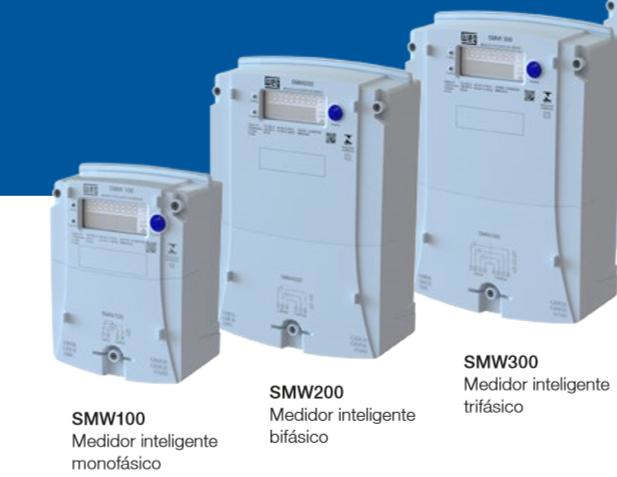
\includegraphics[width=0.7\textwidth]{figuras/medidoresInteligentesSMW.png}
	\caption{Linha de medidores inteligentes SMW}
	\label{fig:medidoresinteligentes}
\end{figure}

\subsection{Automação dos componentes do Biogás}
Como explicado na parte de biogás, para a conversão do gás produzido para energia elétrica será necessário a utilização de um motor Ciclo de Otto, um alternador síncrono, em que o mesmo converte a energia mecânica em energia elétrica, um quadro de transferência automática para sincronização e um medidor de energia elétrica, porém, como medida simplificadora vamos utilizar um grupo gerador, em que este, tem a finalidade de unir o motor Ciclo de Otto e o alternador em apenas um equipamento, formando o seguinte esquema:
\begin{figure}[!h]
	\centering
	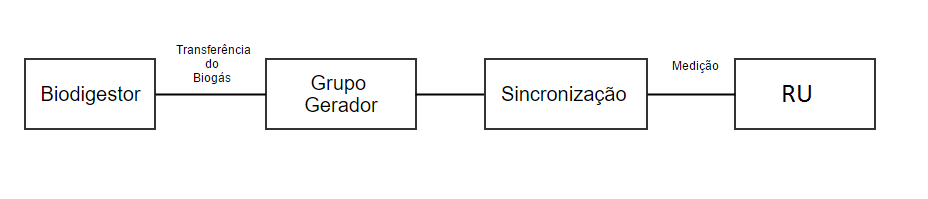
\includegraphics[width=0.75\textwidth]{figuras/ordemFuncBiodigestor.png}
	\caption{Fluxograma ordem de funcionamento}
	\label{fig:funcbiodigestor}
\end{figure}

Para se determinar um grupo gerador eficiente, primeiramente, precisamos calcular a quantidade de biogás que poderá ser gerado considerando apenas a utilização dos 240 kg de lixo orgânicos produzidos diariamente. O processo de decomposição de lixo orgânico dura aproximadamente 3 meses, com isso após o processo de deposição contínua e decomposição, podemos estimar que após 3 meses teremos 12 $m^{3}$ de biogás para uso diário como fonte de energia, considerando que 20 kg de lixo orgânico produza 1 $m^{3}$de biogás. 

Após os cálculos podemos notar que precisaremos de um grupo gerador que consiga consumir os 12 $m^{3}$ de biogás diários.

Com isso podemos definir uma escolha, o gerador BAT - 5000 BIO, da fabricante Branco, de 3,6 kW e com um consumo de 2 $m^{3}$ por hora [11], informados pelo fabricante. A partir desses dados podemos definir quanto de energia se espera gerar utilizando a fórmula:
\begin{equation}
E = P x T
\end{equation}
Em que, $E$ é a energia em kWh, $P$ a potência do gerador e $T$ o tempo de uso. Como possuímos 12 $m^{3}$ de biogás, concluímos então que o gerador será utilizado 6 horas por dia, tendo então uma geração de 21,6 kWh por dia, a ser utilizada pelos aquecedores dos restaurante universitário.
\begin{figure}[!h]
	\centering
	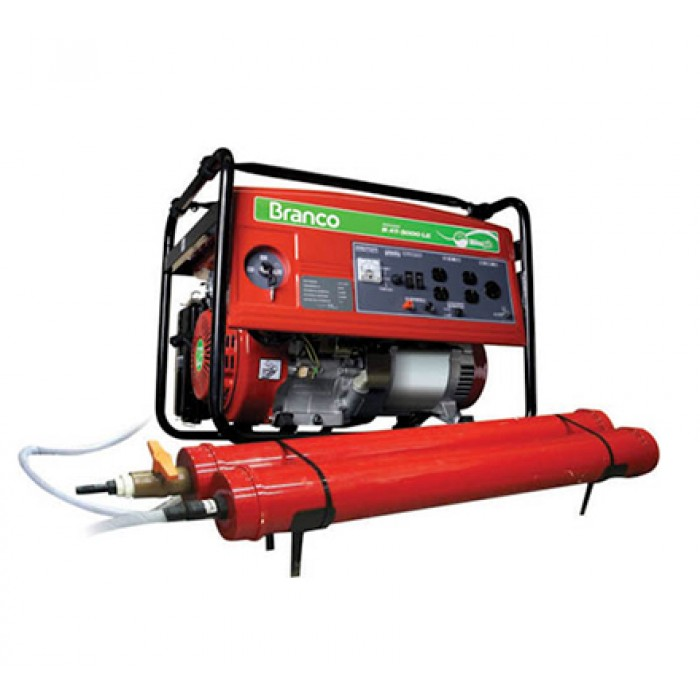
\includegraphics[width=0.7\textwidth]{figuras/geradorBAT.png}
	\caption{Gerador BAT - 5000 BIO [5]}
	\label{fig:geradorbat}
\end{figure}

Vale ressaltar que as saídas do gerador são 220V (fase-neutro) [12], ou seja monofásica, o que nos permite ligar diretamente no quadro de transferência automática e consequentemente distribuir para a cozinha sem a necessidade da utilização de um transformador trifásico para monofásico.

\subsection{Sincronização}
Para a utilização da energia gerada nos equipamentos de aquecimento do restaurante universitário, optamos por utilizar um quadro de transferência automática de transição aberta, que permite fazer a troca do fornecedor primário para o fornecedor secundário (e vice-versa) em momentos de necessidade e pré-programadas. No nosso caso, iremos optar pelas configurações pré-programadas, em que o quadro de transferência automática quando programado o tempo de uso, dá a partida no gerador e o mantém ligado fornecendo energia durante o tempo determinado e gerando assim um desconto relativo. 

Caso os equipamentos que utilizam a energia elétrica ao serem alternadas para a energia dos geradores não possam sofrer nenhum tipo de interrupção, uma possível solução seria a utilização de quadros de transferência automática baseados em tiristores que permitem uma rápida transição que é imperceptível para a maioria das cargas elétricas. 

Os quadros de transferência automática também possuem a finalidade de correção da angulação da fase, frequência e magnitude da tensão caso seja necessário

A escolha do quadro de transferência foi baseada em seu tempo de resposta após a troca da utilização da energia proveniente da concessionária de energia para a do gerador, pela capacidade de conservação do gerador, pois o liga em tempo programado apenas para evitar acúmulo de sujeira que podem comprometer o uso do gerador. Além dos seus parâmetros se encaixar com os fornecidos pelo gerador.

Portanto um modelo que serve como opção é o da marca Strazmaq, modelo QTASTZ-MONO-8K-30A.
\begin{figure}[!h]
	\centering
	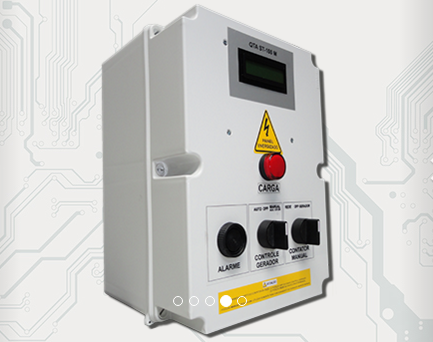
\includegraphics[width=0.7\textwidth]{figuras/quadroStrazmaq.png}
	\caption{Quadro de transferência automática da Strazmaq [6]}
	\label{fig:geradorbat}
\end{figure}

\subsection{Softwares de gerenciamento}
A importância da informação para a tomada de decisões nas organizações tem impulsionado o desenvolvimento dos sistemas de processamento de informações. Algumas ferramentas importantes para esse processo são: processadores de texto (editoração eletrônica), planilhas (cálculos com tabelas de valores) e Sistemas de Gerenciamento de Bancos de Dados - SGBDs (armazenamento de grandes volumes de dados, estruturados em registros e tabelas, com recursos para acesso e processamento das informações) \cite{rocha2015importancia}.

Por definição, banco de dados é uma coleção de dados interrelacionados, representando informações sobre um domínio específico. Por exemplo: lista telefônica, controle do acervo de uma biblioteca, sistema de controle dos recursos humanos de uma empresa. 

Sistema de Gerenciamento de Bancos de Dados (SGBD) é um conceito diferente, mas que se relaciona com banco de dados. Por definição, é um software com recursos específicos para facilitar a manipulação das informações dos bancos de dados e o desenvolvimento de programas aplicativos.

Para o projeto em desenvolvimento, é necessário possuir e consultar uma base de dados ligada a distribuição de energia elétrica. Também é importante desenvolver um ambiente de interface homem-máquina que inclui algumas aplicações, como análise e otimização de redes elétricas, cálculo e balanço de perdas técnicas e não técnicas.

Além disso, é interessante existir um módulo encarregado da gestão de eventos causados por alterações topológicas na rede elétrica. Tal sistema registraria os blecautes, mostraria graficamente o estado de energização ou não energização da rede elétrica e permitiria simulações de manobras e falhas. 

A melhor solução encontrada foi o sistema ActionoGRID, da empresa Spin Engenharia de Automação, que é um conjunto completo de módulos de software com diversas funcionalidades que facilitam o processo de geração, manutenção e operação da rede de distribuição de energia elétrica.

O software SCADA utilizado nesse sistema é o Action.NET que faz a aquisição de dados e controle de supervisão do processo controlado. Trabalha em plataforma de 64 bits, que suporta todos os protocolos da área elétrica, o que anula o risco de não compatibilidade entre os dispositivos da automação.

Tal sistema possui uma infra-estrutura flexível para gerenciamento de dados em tempo real, com aplicações ao setor elétrico, em geração, transmissão e distribuição, energia renovável, e outras plantas distribuídas como o gerenciamento de distribuição de água e sistemas de automação predial. Essas características suprem as principais demandas de automação e análise de dados de um sistema smart grid em ambiente universitário.

Além disso, inclui um banco de dados com os tags em tempo real, os níveis hierárquicos de ativos e modelos, alarmes e eventos, historiador, receitas, consultas SQL e acesso de dados, elaboração de relatórios, lógicas em scripts em linguagem .NET, cliente e servidor OPC, WCF e protocolos nativos da indústria, gráficos dinâmicos criados em WPF e acessível a partir de desktops, clientes remotos inteligentes, navegador e iOS clientes nativos em iPads e iPhones.
\begin{figure}[!h]
	\centering
	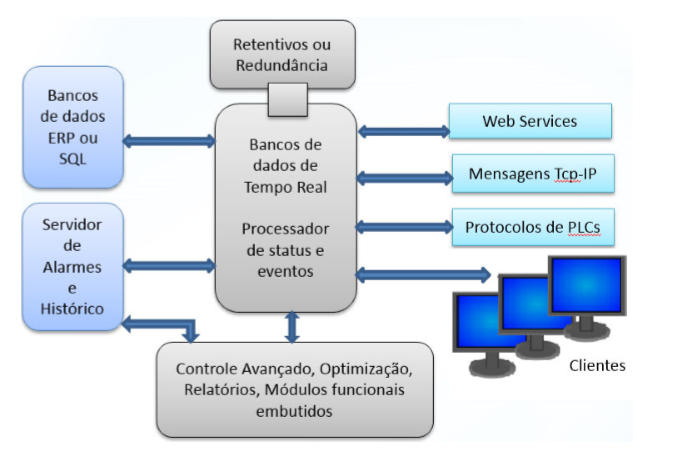
\includegraphics[width=0.75\textwidth]{figuras/bancoDados.png}
	\caption{Esquematização do sistema de banco de dados}
	\label{fig:bancodados}
\end{figure}

Action.NET suporta acesso SQL, Web-Services, XML e outras interfaces de intercâmbio de dados para fornecer informções para ferramentas de relatórios externos. Além disso, ele tem o seu próprio editor de relatório.

O Action.NET pode ser aplicado em diferentes cenários e topologias de rede. As aplicações mais comuns, desde o chão de fábrica até a TI, incluem[Manual – Action.NET: Manual do Usuário]:
\begin{itemize}
\item Painel HMI local ou dispositivo embutido, funcionando para aquisição de dados por protocolos nativos e operação local;
\item Servidor OPC e gateway de dados;
\item Supervisão e sistema SCADA em ilhas de automação;
\item Servidor Central para Centros de Operações e Controle Integrado de Salas;
\item Servidor de Dados prontos para “cloud” independente da fonte da camada de apresentação;
\item PMIS - painel em tempo real e Plant Information; 
\item Gestão de Aplicações de Informações de Plantas.
\end{itemize}

Por fim, os requisitos técnicos para se utilizar o sistema são [Manual – Action.NET: Manual do Usuário ]:
\begin{itemize}
\item Microsoft dotNET Framework v4.0;
\item Sistemas operacionais: qualquer sistema operacional capaz de executar o Microsoft NET Framework 4.0 ou máquinas virtuais compatíveis com o Microsoft NET Framework;
\item Windows 7, Windows 8, Windows Vista, Windows Server 2008 e Windows Server 2012 todos vêm com a \item Microsoft. Instalado Net;
\item Memória RAM: Runtime 1 GB; Engenharia 2 GB;
\item Espaço em disco-150 MB;
\item Resolução da tela:
	\begin{itemize}
	\item Para o desenvolvimento de aplicações de mínima de 1024 x 768;
	\item Para a aplicação de tempo real: As Telas são independentes da resolução, para que você possa criar aplicações que vão desde pequenos HMI de 6” até grandes monitores de alta definição;
	\end{itemize}
\item Para ter acesso às instalações baseadas na web, Internet Explorer v8 ou posterior.
\end{itemize}